\section{Regression accuracy}
The plot in \figref{fig:regressionOutputVsInput} depicts the actual data superimposed on the estimated data from the regressors. 

\begin{figure}[H]
	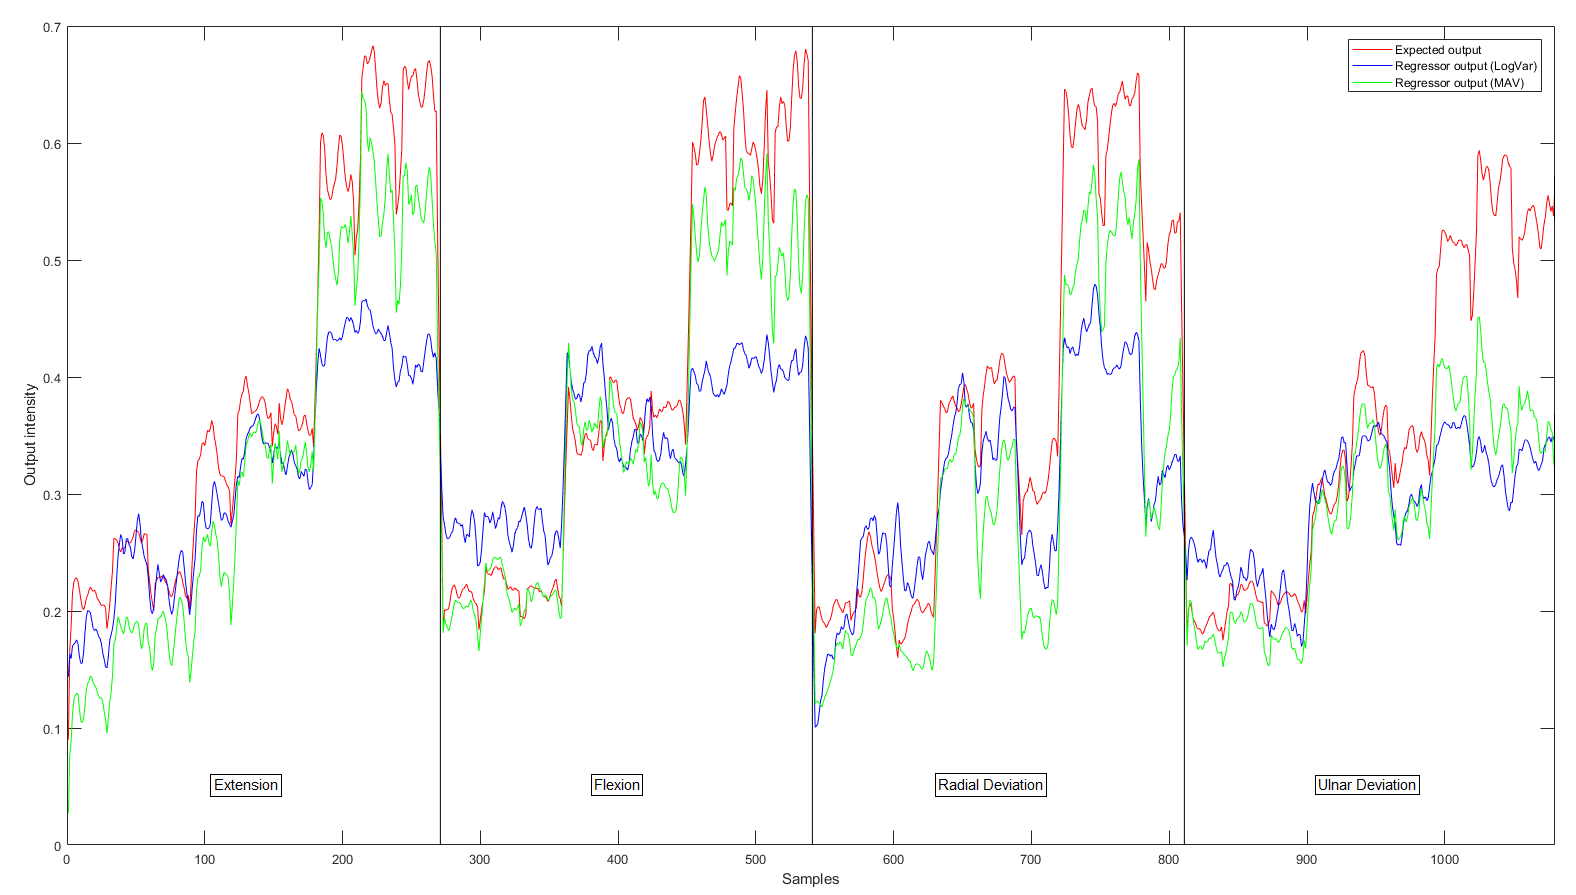
\includegraphics[width=0.7\textwidth]{figures/results/regressionOutputVsInput}  %<--but is not needed.
	\caption{Plot of the actual data, red plot, superimposed on the regression outputs from the logarithmic variance and MAV features for the four hand gestures, which is the blue and green plot respectively. Each segmentation of the hand gestures has the same sample size.}
	\label{fig:regressionOutputVsInput}  %<--give the figure a label, so you can reference!
\end{figure}

A quantitatively examination of the plot shows that regression on MAV features yields a more accurate output than regression on the logarithmic variance feature, whereas both estimates yield inaccurate fitting in the high intensities. However, both estimates yield inaccurate fitting in the high intensities compared to the lower intensities, especially in the ulnar deviation movement.
  


Calculating the RMSE of the regressors for the MAV and logarithmic variance features of the training data across all subjects, yields the results depicted in \figref{fig:gimmeThemRMSEBars}. The overall mean of the RMSE of MAV is 0.0867 with a standard deviation of $\pm 0.0310$, where the highest mean of a regressor is 0.0410 and the highest standard deviation is $\pm 0.0975$. The overall mean of the RMSE of the logarithmic variance is 0.1047 with a standard deviation of $\pm 0.0273$, where the highest mean of a regressor is 0.0386 and the highest standard deviation is $\pm 0.1097$. MAV then yields a lower mean RMSE than the logarithmic variance, where the logarithmic variance has a lower standard deviation than MAV. 

\begin{figure}[H]
	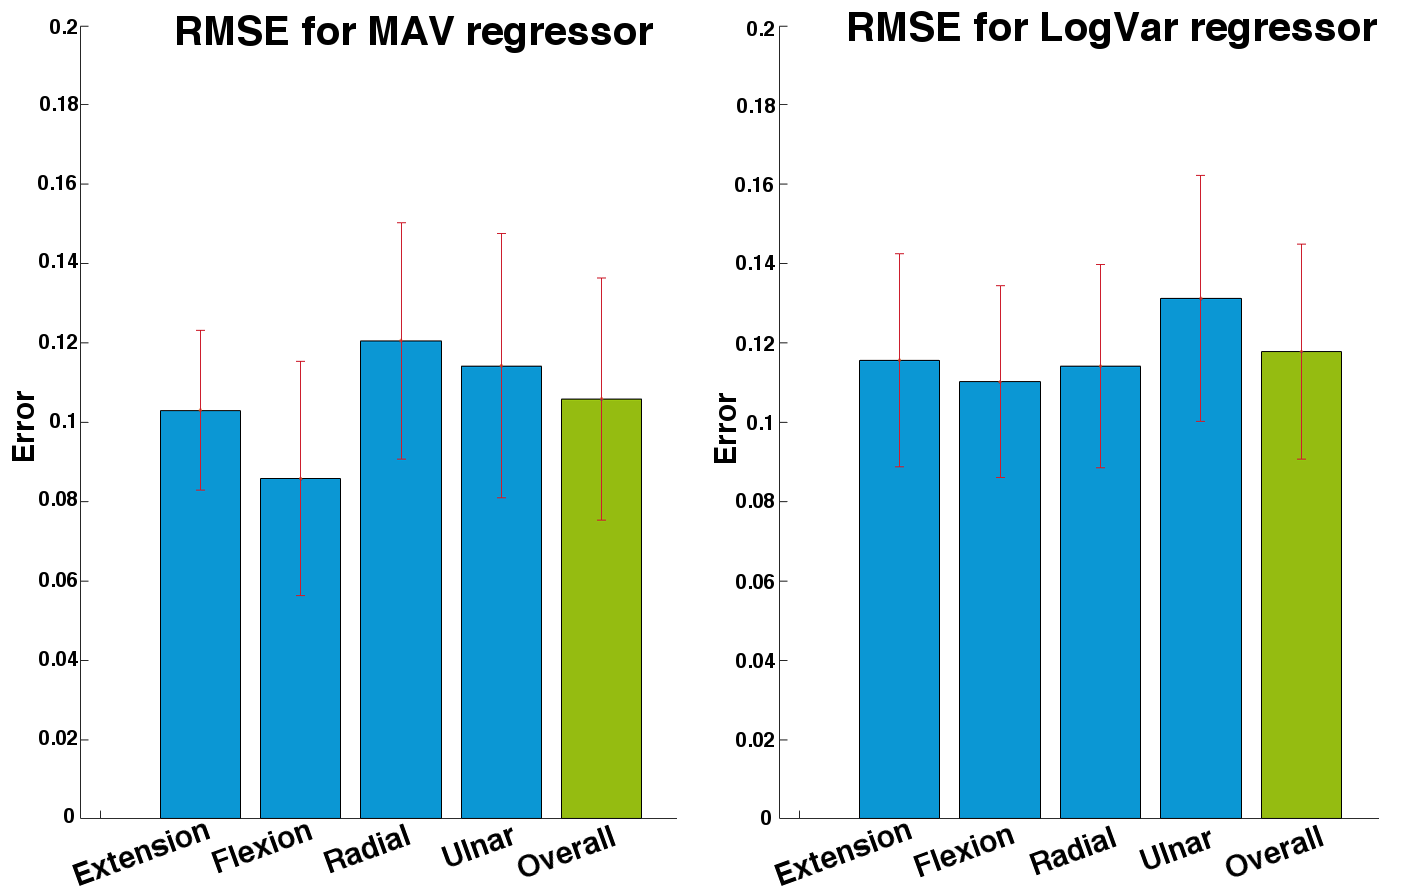
\includegraphics[width=.7\textwidth]{figures/results/gimmeThemRMSEBars}  %<--but is not needed.
	\caption{Bar plot of the error of MAV and the logarithmic variance features for the four hand gestures. The bar chart illustrates the mean error and the error bar illustrates the standard deviation}
	\label{fig:gimmeThemRMSEBars}  %<--give the figure a label, so you can reference!
\end{figure}